\documentclass{article}
\usepackage{flowchart}
\usepackage{tikz}
\usetikzlibrary{shapes,arrows,chains}
\begin{document}
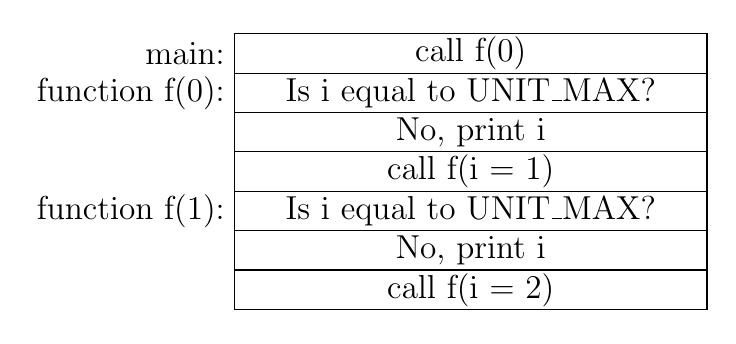
\begin{tikzpicture}[>=latex']
  \draw (0, 0)--(0,-.5cm)--(6cm, -.5cm)--(6cm, 0)--cycle;
  \node[anchor=east] at (0, -.25cm){\large main:};
  \draw (3cm, -.25cm) node {\large call f(0)};
  \draw (0, -.5cm)--(0, -1cm)--(6cm, -1cm)--(6cm, -.5cm)--cycle;
  \node[anchor=east] at (0, -.75cm){\large function f(0):};
  \draw (3cm, -.75cm) node {\large Is i equal to UNIT\_MAX?};
  \draw (0, -1cm)--(0, -1.5cm)--(6cm, -1.5cm)--(6cm, -1cm)--cycle;
  \node at (3cm, -1.25cm){\large No, print i};
  \draw (0, -1.5cm)--(0, -2cm)--(6cm, -2cm)--(6cm, -1.5cm)--cycle;
  \draw (3cm, -1.75cm) node {\large call f(i = 1)};
  \draw (0, -2cm)--(0, -2.5cm)--(6cm, -2.5cm)--(6cm, -2cm)--cycle;
  \node[anchor=east] at (0, -2.25cm){\large function f(1):};
  \draw (3cm, -2.25cm) node {\large Is i equal to UNIT\_MAX?};
  \draw (0, -2.5cm)--(0, -3cm)--(6cm, -3cm)--(6cm, -2.5cm)--cycle;
  \node at (3cm, -2.75cm){\large No, print i};
  \draw (0, -3cm)--(0, -3.5cm)--(6cm, -3.5cm)--(6cm, -3cm)--cycle;
  \draw (3cm, -3.25cm) node {\large call f(i = 2)};
  
\end{tikzpicture}
\end{document}
